\section{Unos i uređivanje podataka}

Kako bi sustav bio dinamičan i ažuran, aplikacija omogućuje ovlaštenim korisnicima kreiranje i uređivanje svih hijerarhijskih razina podataka, od penjačke lokacije do pojedinačnih penjačkih smjerova.

\subsection{Dodavanje i uređivanje penjačkih lokacija}

Na korisničkom profilu omogućeno je kreiranje nove penjačke lokacije u izborniku u gornjem desnom kutu pregleda. Na web aplikaciji ta opcija se nalazi u navigacijskoj traci u postavkama korisničkog izbornika. Kreiranja novog penjališta nije dostupna svim korisnicima, već je ograničena na one s posebnim ovlastima, a to su administratori sustava i verificirani korisnici (eng. \textit{creators}). 
Ovlašteni korisnik odabirom ove opcije pristupa formi za unos nove penjačke lokacije. Potrebno je unijeti naziv penjališta, opcionalni opis koji može sadržavati sadržavati informacije o povijesti regije ili slične zanimljivosti, te naziv šire geografske lokacije. Ime geografske lokacije korisnik može samostalno dodati, no ako ne postoji, aplikacija će automatski dodati naziv geografske lokacije na temelju lokacije penjačke lokacije. Ključno, korisnik može dodati jednu ili više fotografija koje vizualno predstavljaju penjalište. Nakon unosa svih podataka, novo penjalište se stvara u sustavu i postaje dostupno svim korisnicima.

\begin{figure}[H]
    \centering
    \begin{subfigure}[b]{0.31\textwidth}
        \centering
        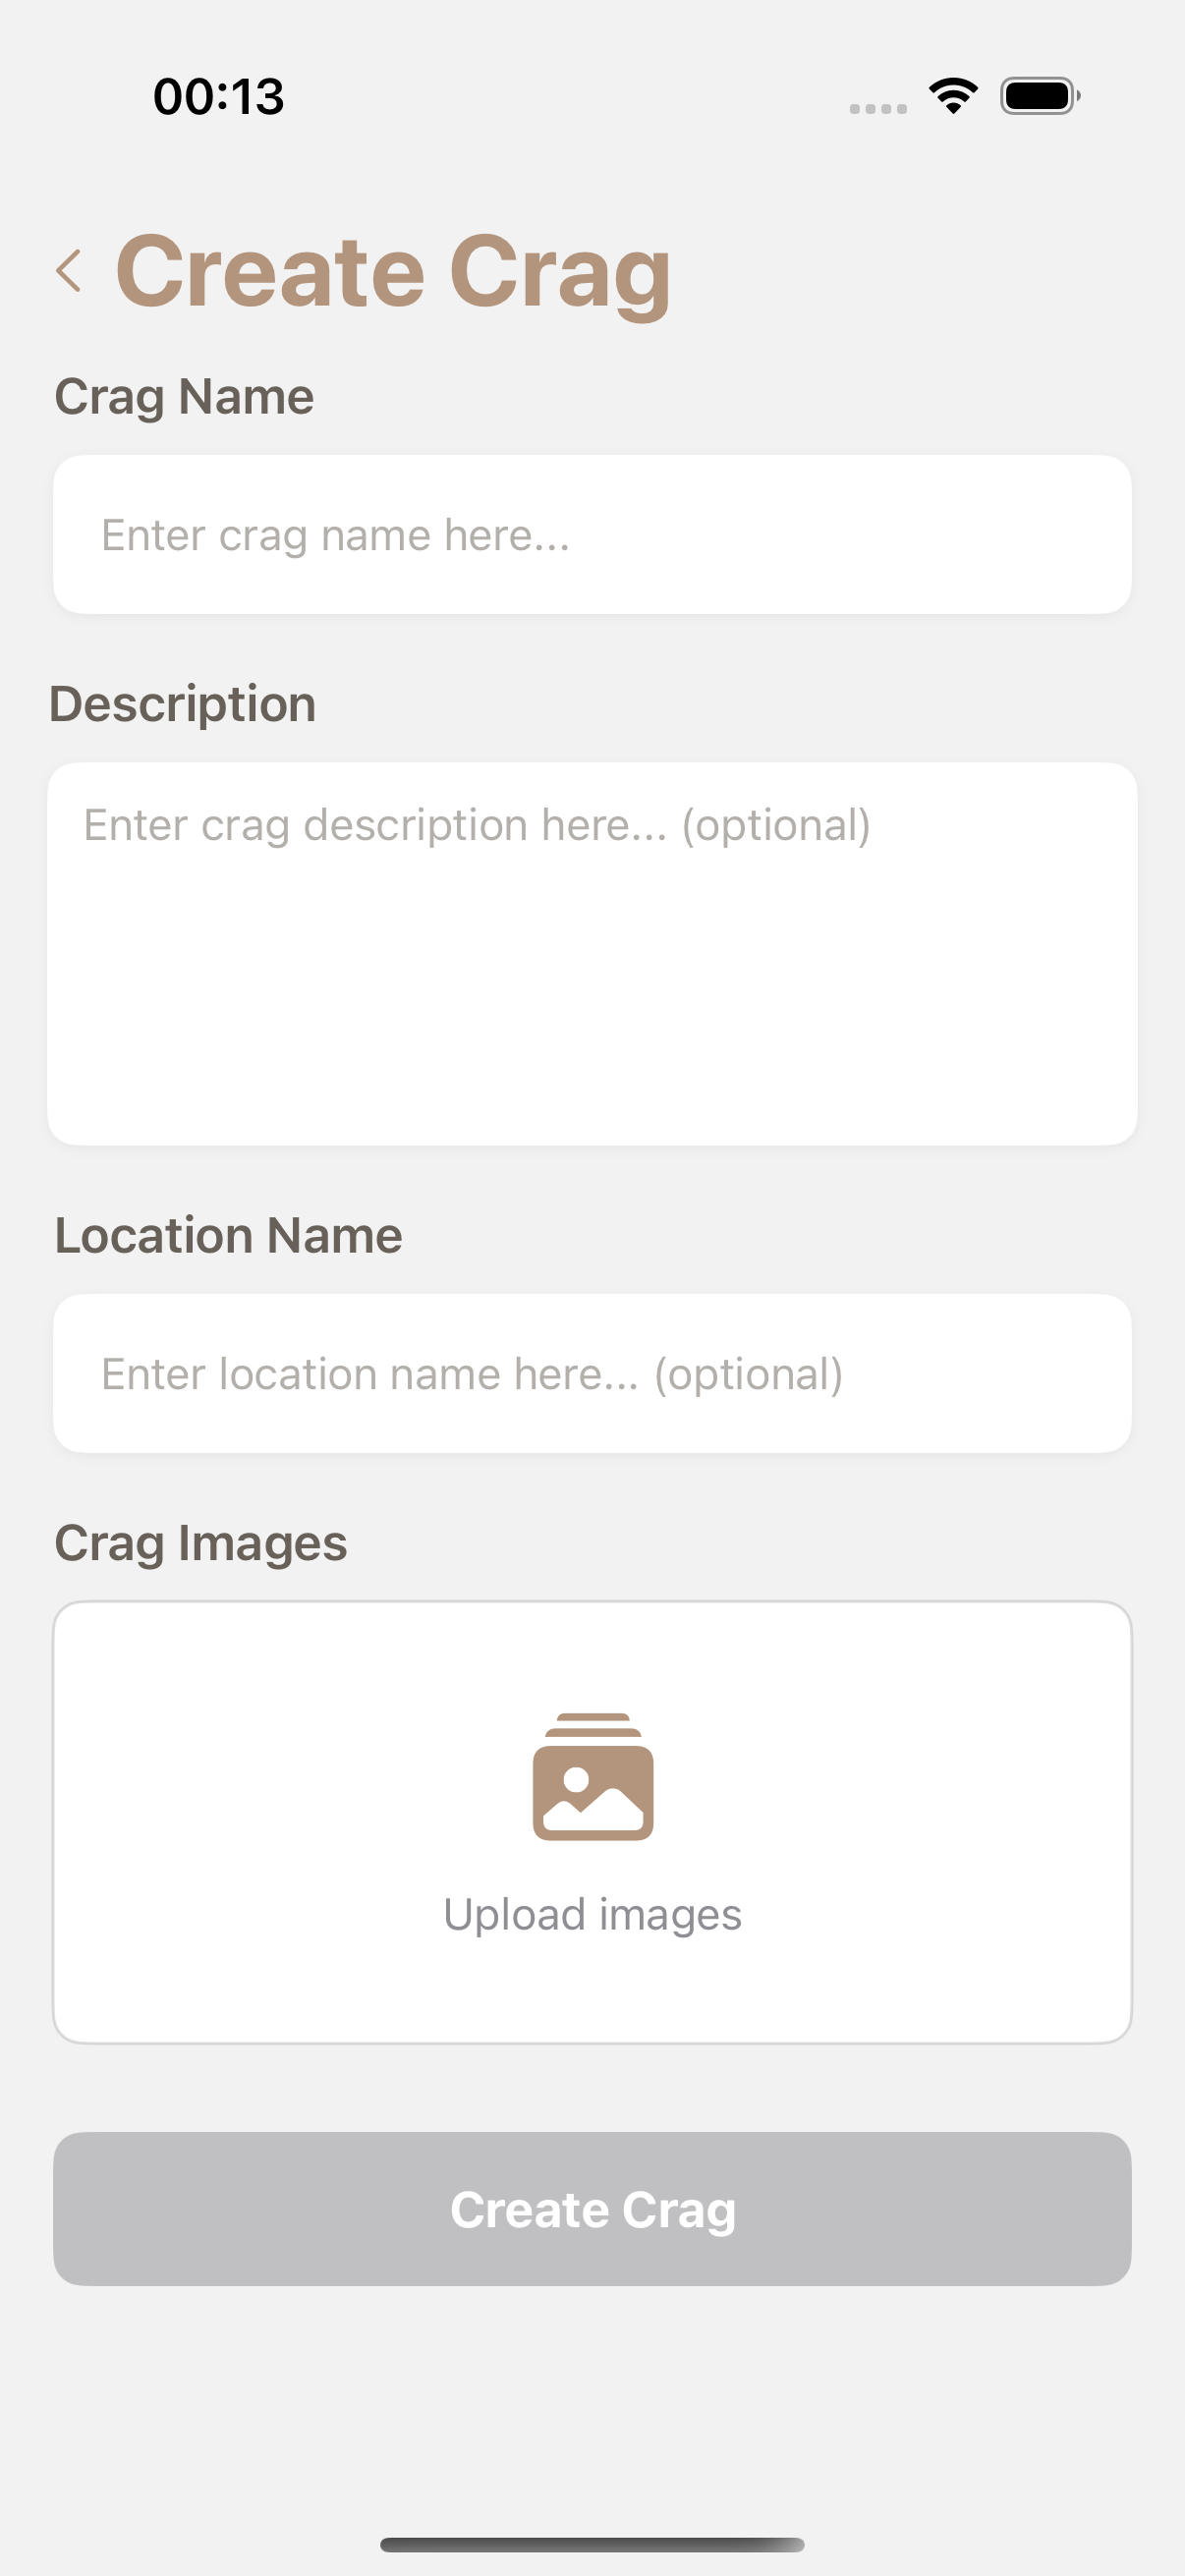
\includegraphics[width=\textwidth]{images/implementacija/editing-options/create_crag.png}
        \caption{Mobilna aplikacija}
        \label{fig:dodavanje_lokacije_mob}
    \end{subfigure}
    \hfill
    \begin{subfigure}[b]{0.6\textwidth}
        \centering
        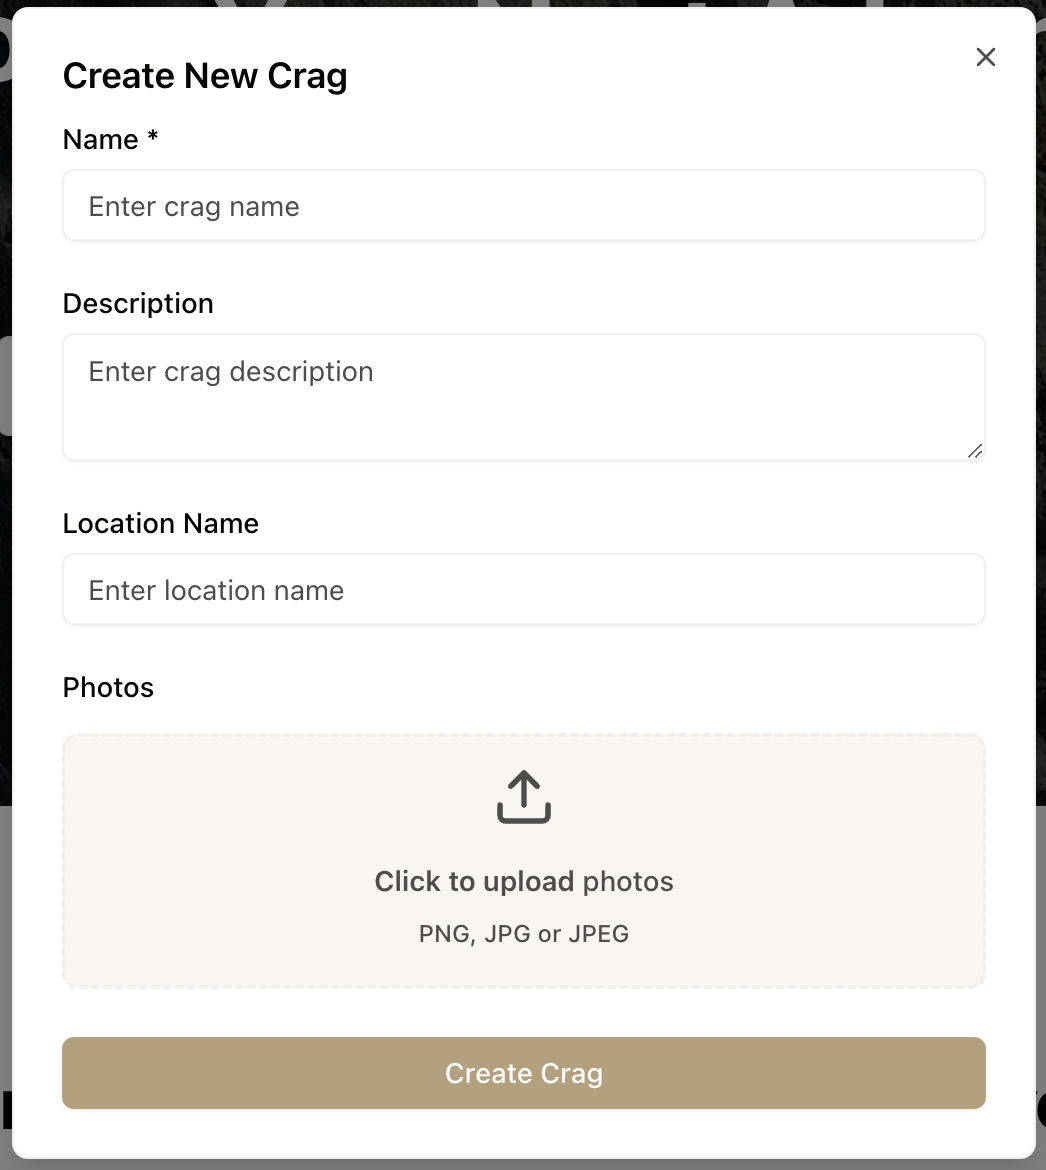
\includegraphics[width=\textwidth]{images/implementacija/web/editing-options/create-crag.png}
        \caption{Web aplikacija}
        \label{fig:dodavanje_lokacije_web}
    \end{subfigure}
    \caption{Dodavanje nove penjačke lokacije}
    \label{fig:dodavanje_lokacije}
\end{figure}

Osim kreiranja novih, ovlašteni korisnicim imaju mogućnost i uređivanja postojećih panjačkih lokacija. Pristup ovoj funkcionalnosti omogućen je kroz izbornik na zaslonu s detaljnim pregledom penjačke lokacije. Sučelje za uređivanje omogućuje promjenu svih prethodno unesenih podataka, uključujući naziv, opis i naziv geografske lokacije. Korisnici također mogu upravljati galerijom fotografija, dodajući nove ili uklanjajući postojeće slike. 

\begin{figure}[H]
    \centering
    \begin{subfigure}[b]{0.36\textwidth}
        \centering
        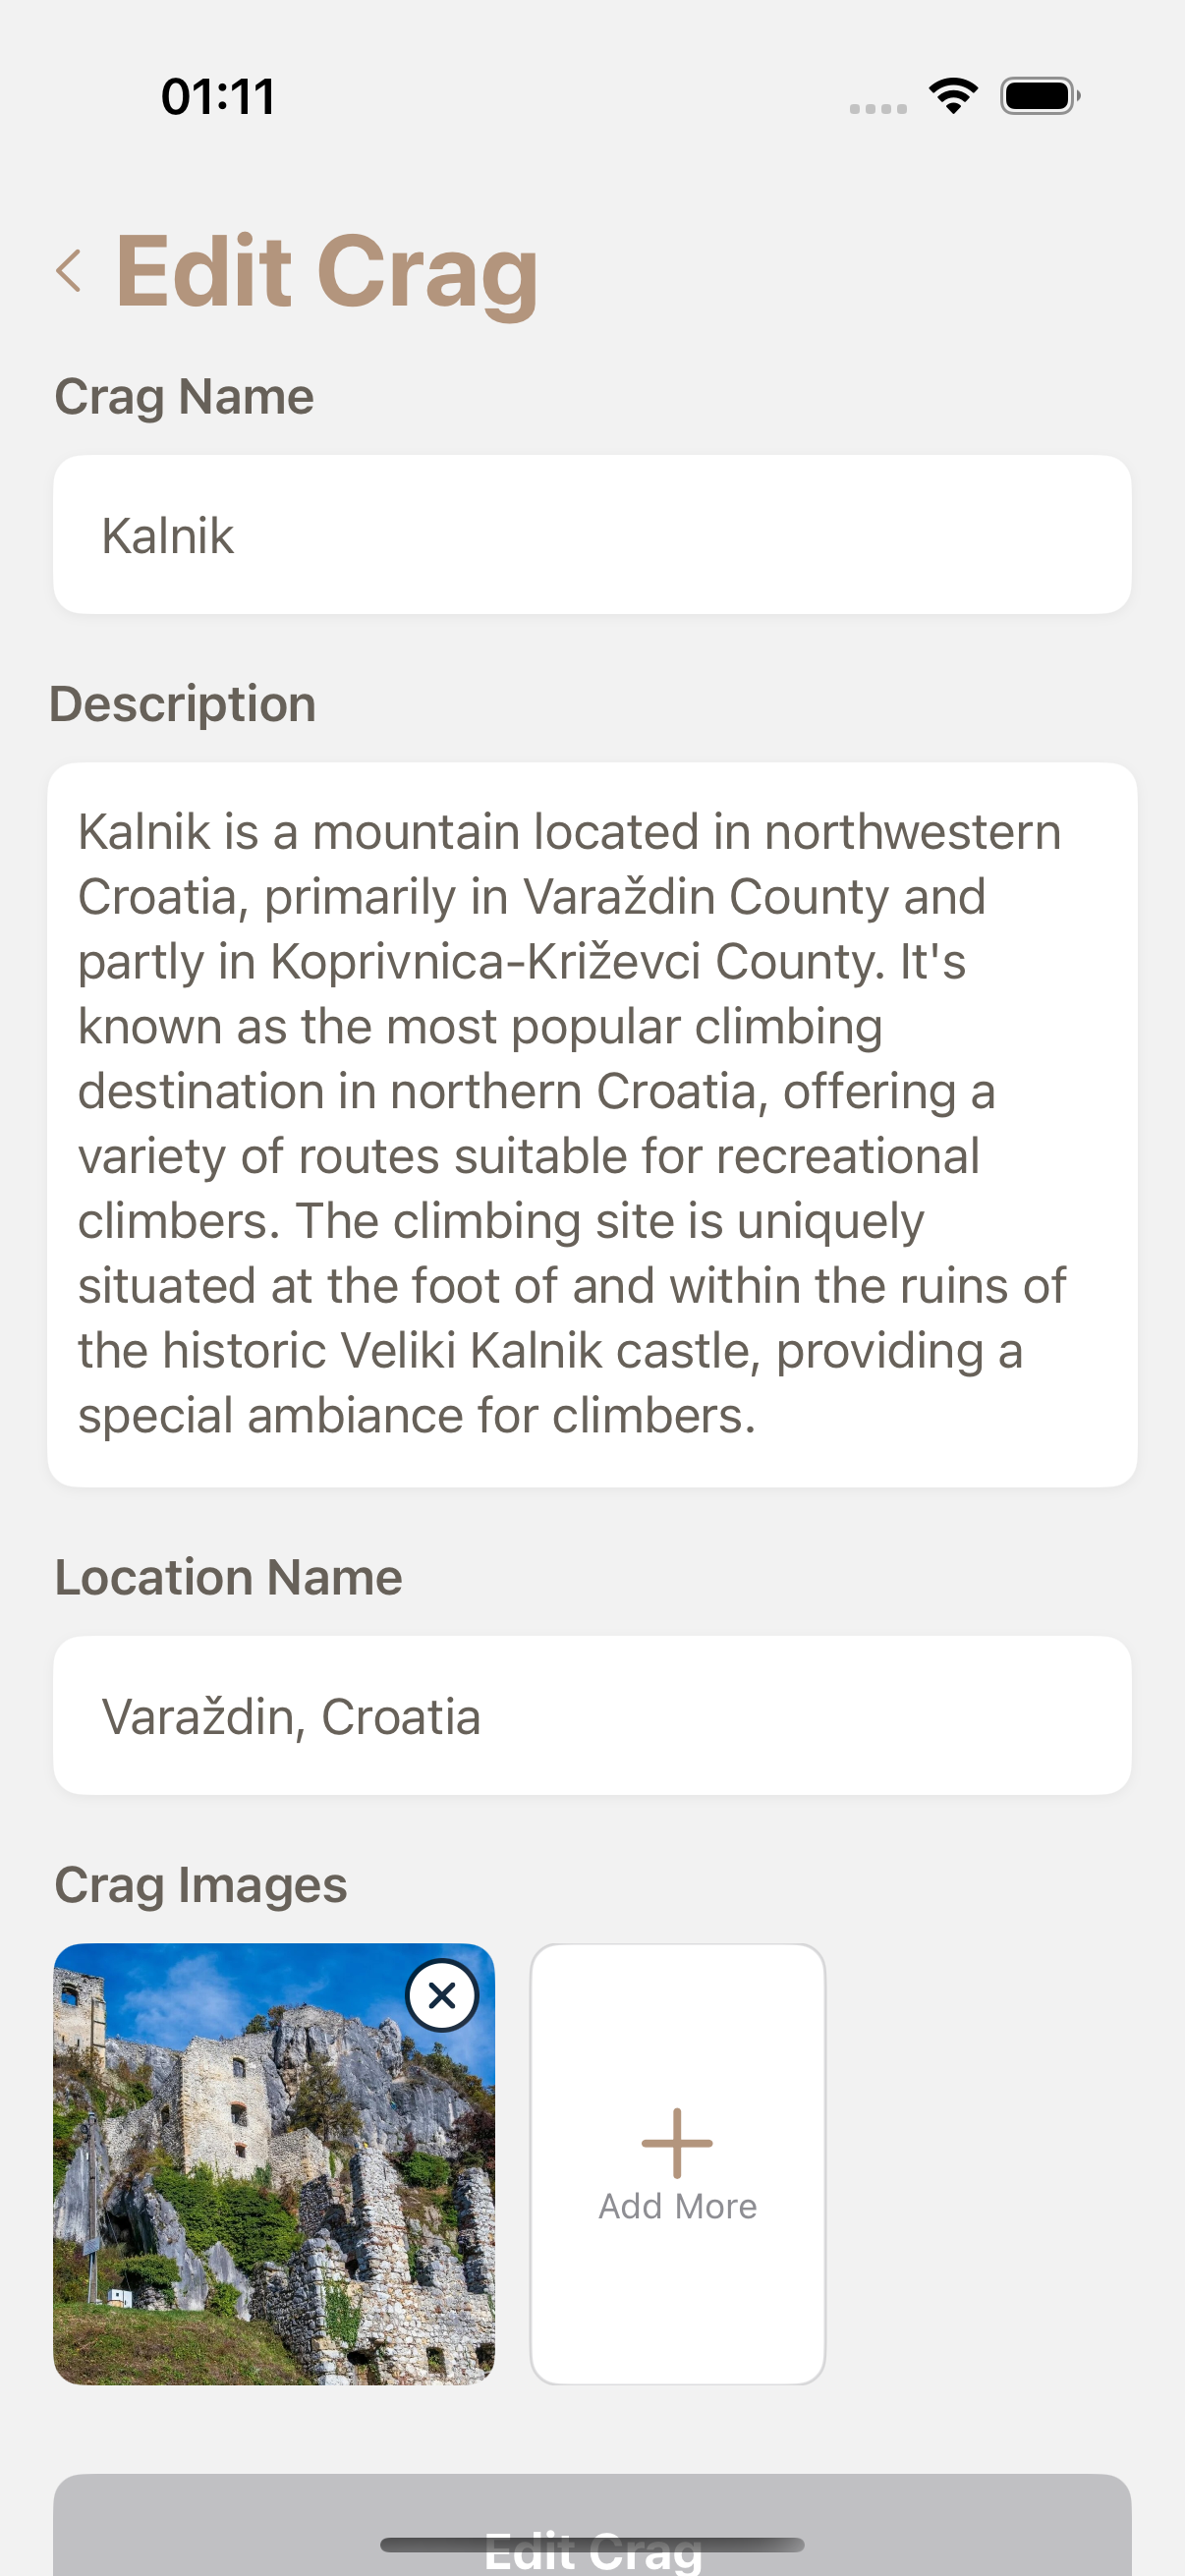
\includegraphics[width=\textwidth]{images/implementacija/editing-options/edit-crag.png}
        \caption{Mobilna aplikacija}
        \label{fig:dodavanje_lokacije_mob}
    \end{subfigure}
    \hfill
    \begin{subfigure}[b]{0.47\textwidth}
        \centering
        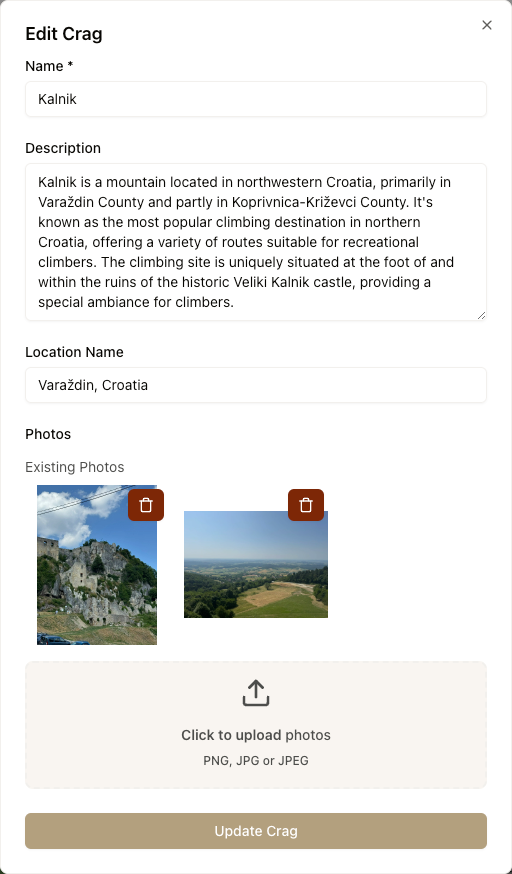
\includegraphics[width=\textwidth]{images/implementacija/web/editing-options/edit-crag.png}
        \caption{Web aplikacija}
        \label{fig:dodavanje_lokacije_web}
    \end{subfigure}
    \caption{Dodavanje nove penjačke lokacije}
    \label{fig:dodavanje_lokacije}
\end{figure}

\subsection{Upravljanje korisničkim ovlastima}

Kako bi se osigurala kontrola nad unosom i uređivanjem podataka, a istovremeno omogućio doprinos više ljudi, sustav implementira mehanizam za upravljanje korisničkim ovlastima na razini pojedinog penjališta. Ovoj funkcionalnosti imaju pristup samo vlasnici penjališta i administratori sustava putem izbornika na zaslonu s detaljnim pregledom penjačke lokacije. Pristupom pregledu za upravljanje ovlastima prikazuje se popis svih korisnika koji trenutno imaju ili mogu dobiti dozvole za uređivanje sadržaja na tom specifičnom penjalištu. Sučelje omogućuje pretragu korisnika po korisničkom imenu te odabir jednog ili više korisnika kojima se žele dodijeliti ili oduzeti ovlasti. Time odabrani korisnik dobiva prava uređivanja penjačkog smjera bez davanja potpunih administrativnih prava.

\begin{figure}[H]
    \centering
    \begin{subfigure}[b]{0.36\textwidth}
        \centering
        
\includegraphics[width=\textwidth]{images/implementacija/editing-options/manage-users.png}
        \caption{Mobilna aplikacija}
        \label{fig:upravljanje_ovlastima_mob}
    \end{subfigure}
    \hfill
    \begin{subfigure}[b]{0.6\textwidth}
        \centering
        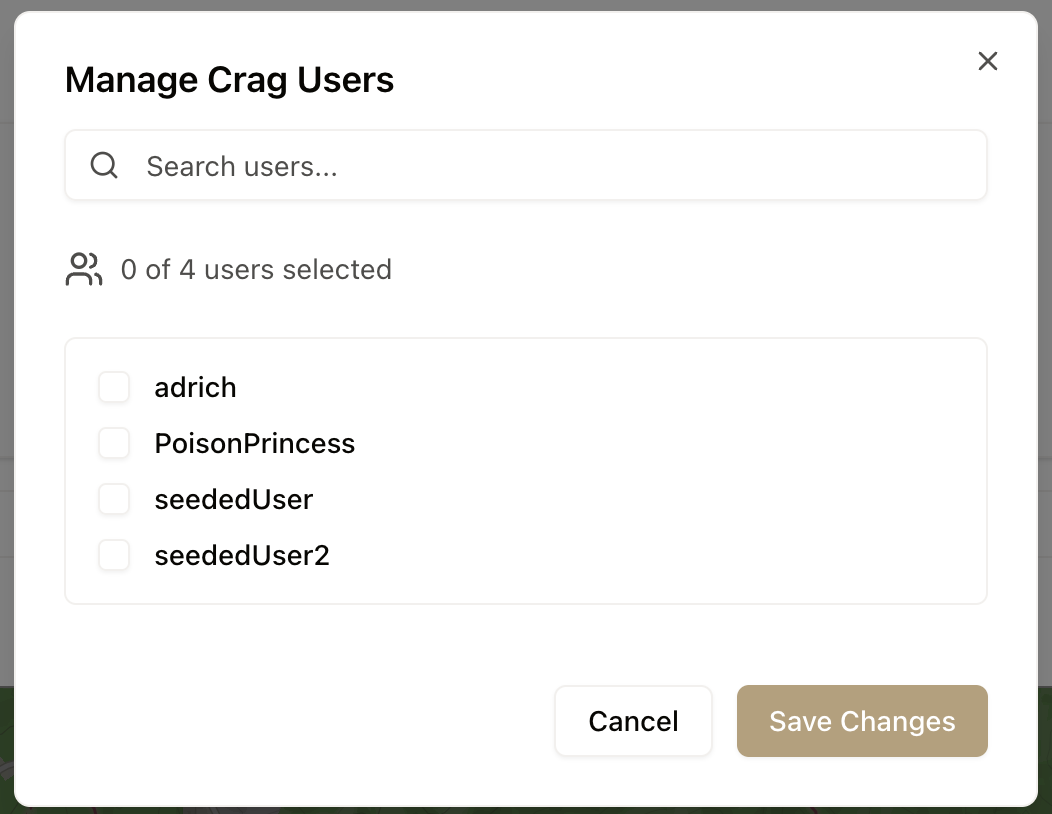
\includegraphics[width=\textwidth]{images/implementacija/web/editing-options/manage-users.png}
        \caption{Web aplikacija}
        \label{fig:upravljanje_ovlastima_web}
    \end{subfigure}
    \caption{Upravljanje korisničkim ovlastima}
    \label{fig:upravljanje_ovlastima}
\end{figure}


\subsection{Dodavanje i uređivanje sektora}

Unutar svake penjačke lokacije, ovlašteni korisnici mogu dalje strukturirati sadržaj kreiranjem i uređivanjem sektora. Pristup opciji za dodavanje nalazi se u izborniku na zaslonu s detaljnim pregledom penjačke lokacije. Forma za unos novog sektora zahtijeva od korisnika unos naziva sektora i opcionalnog opisa, koji može sadržavati specifične informacije koje su specifične za sektore te ostale relevantne informacije. Osim naziva zahtjeva se i upis lokacije u obliku koordinata. Pregledi taj proces olakšavaju uporabom geografske karte, koja omogućuje korisniku da odabere lokaciju sektora na karti ili pretraživanjem po nazivu lokacije. Kao i kod penjačke lokacije, moguće je dodati jednu ili više fotografija koje vizualno predstavljaju sektor.

\begin{figure}[H]
    \centering
    \begin{subfigure}[b]{0.36\textwidth}
        \centering
        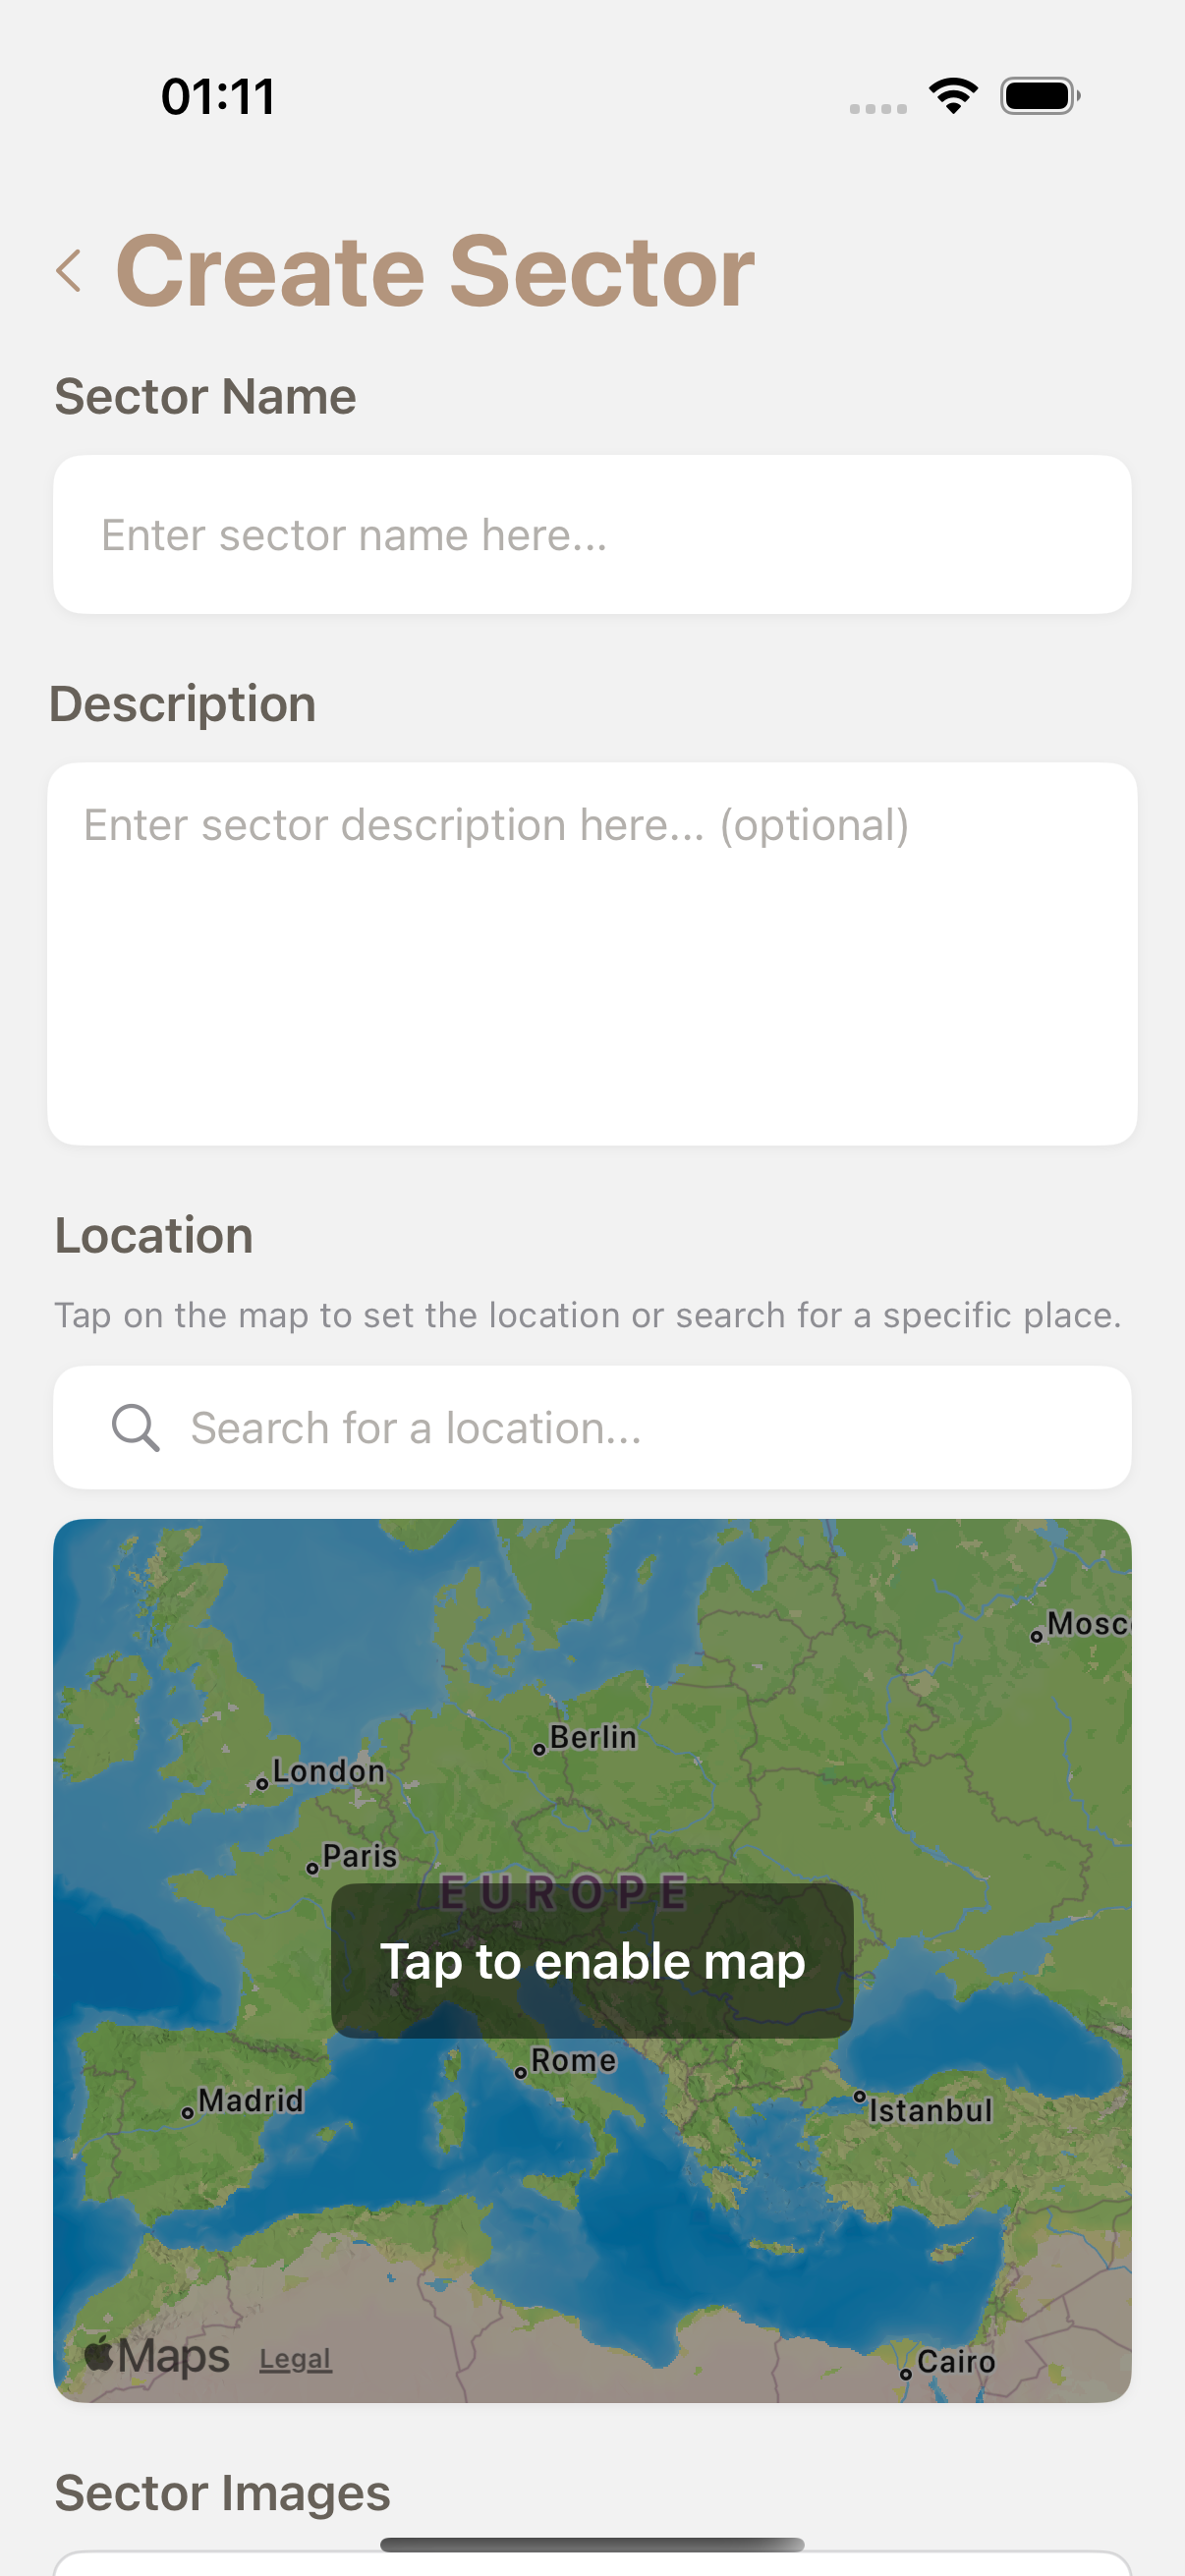
\includegraphics[width=\textwidth]{images/implementacija/editing-options/create-sector.png}
        \caption{Mobilna aplikacija}
        \label{fig:dodavanje_sektora_mob}
    \end{subfigure}
    \hfill
    \begin{subfigure}[b]{0.45\textwidth}
        \centering
        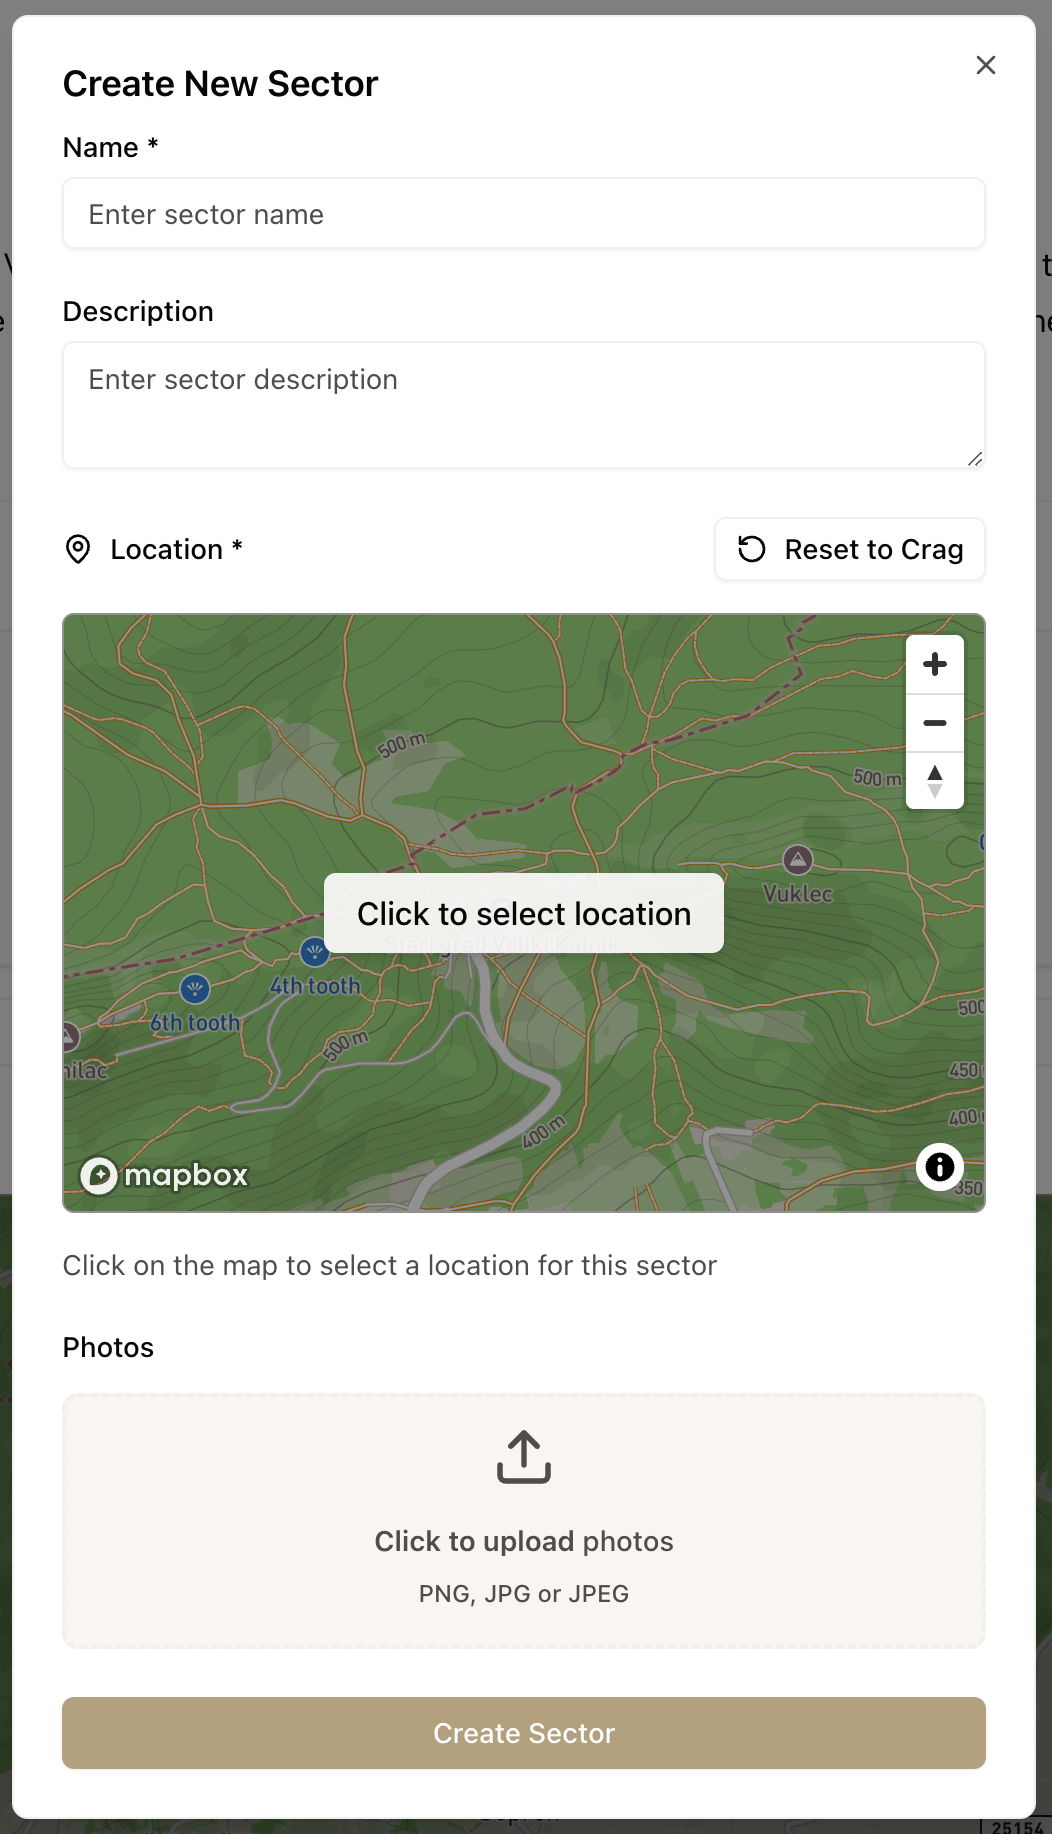
\includegraphics[width=\textwidth]{images/implementacija/web/editing-options/create-sector.png}
        \caption{Web aplikacija}
        \label{fig:dodavanje_sektora_web}
    \end{subfigure}
    \caption{Dodavanje novog sektora}
    \label{fig:dodavanje_sektora}
\end{figure}

Postojeći sektori mogu se uređivati na sličan način. Odabirom određenog sektora, korisniku se prikaže izbornik u kojem se nalazi opcija za uređivanje sektora. Forma omogućuje uređivanje  naziva, opisa, lokaciju i galeriju fotografija.

\begin{figure}[H]
    \centering
    \begin{subfigure}[b]{0.38\textwidth}
        \centering
        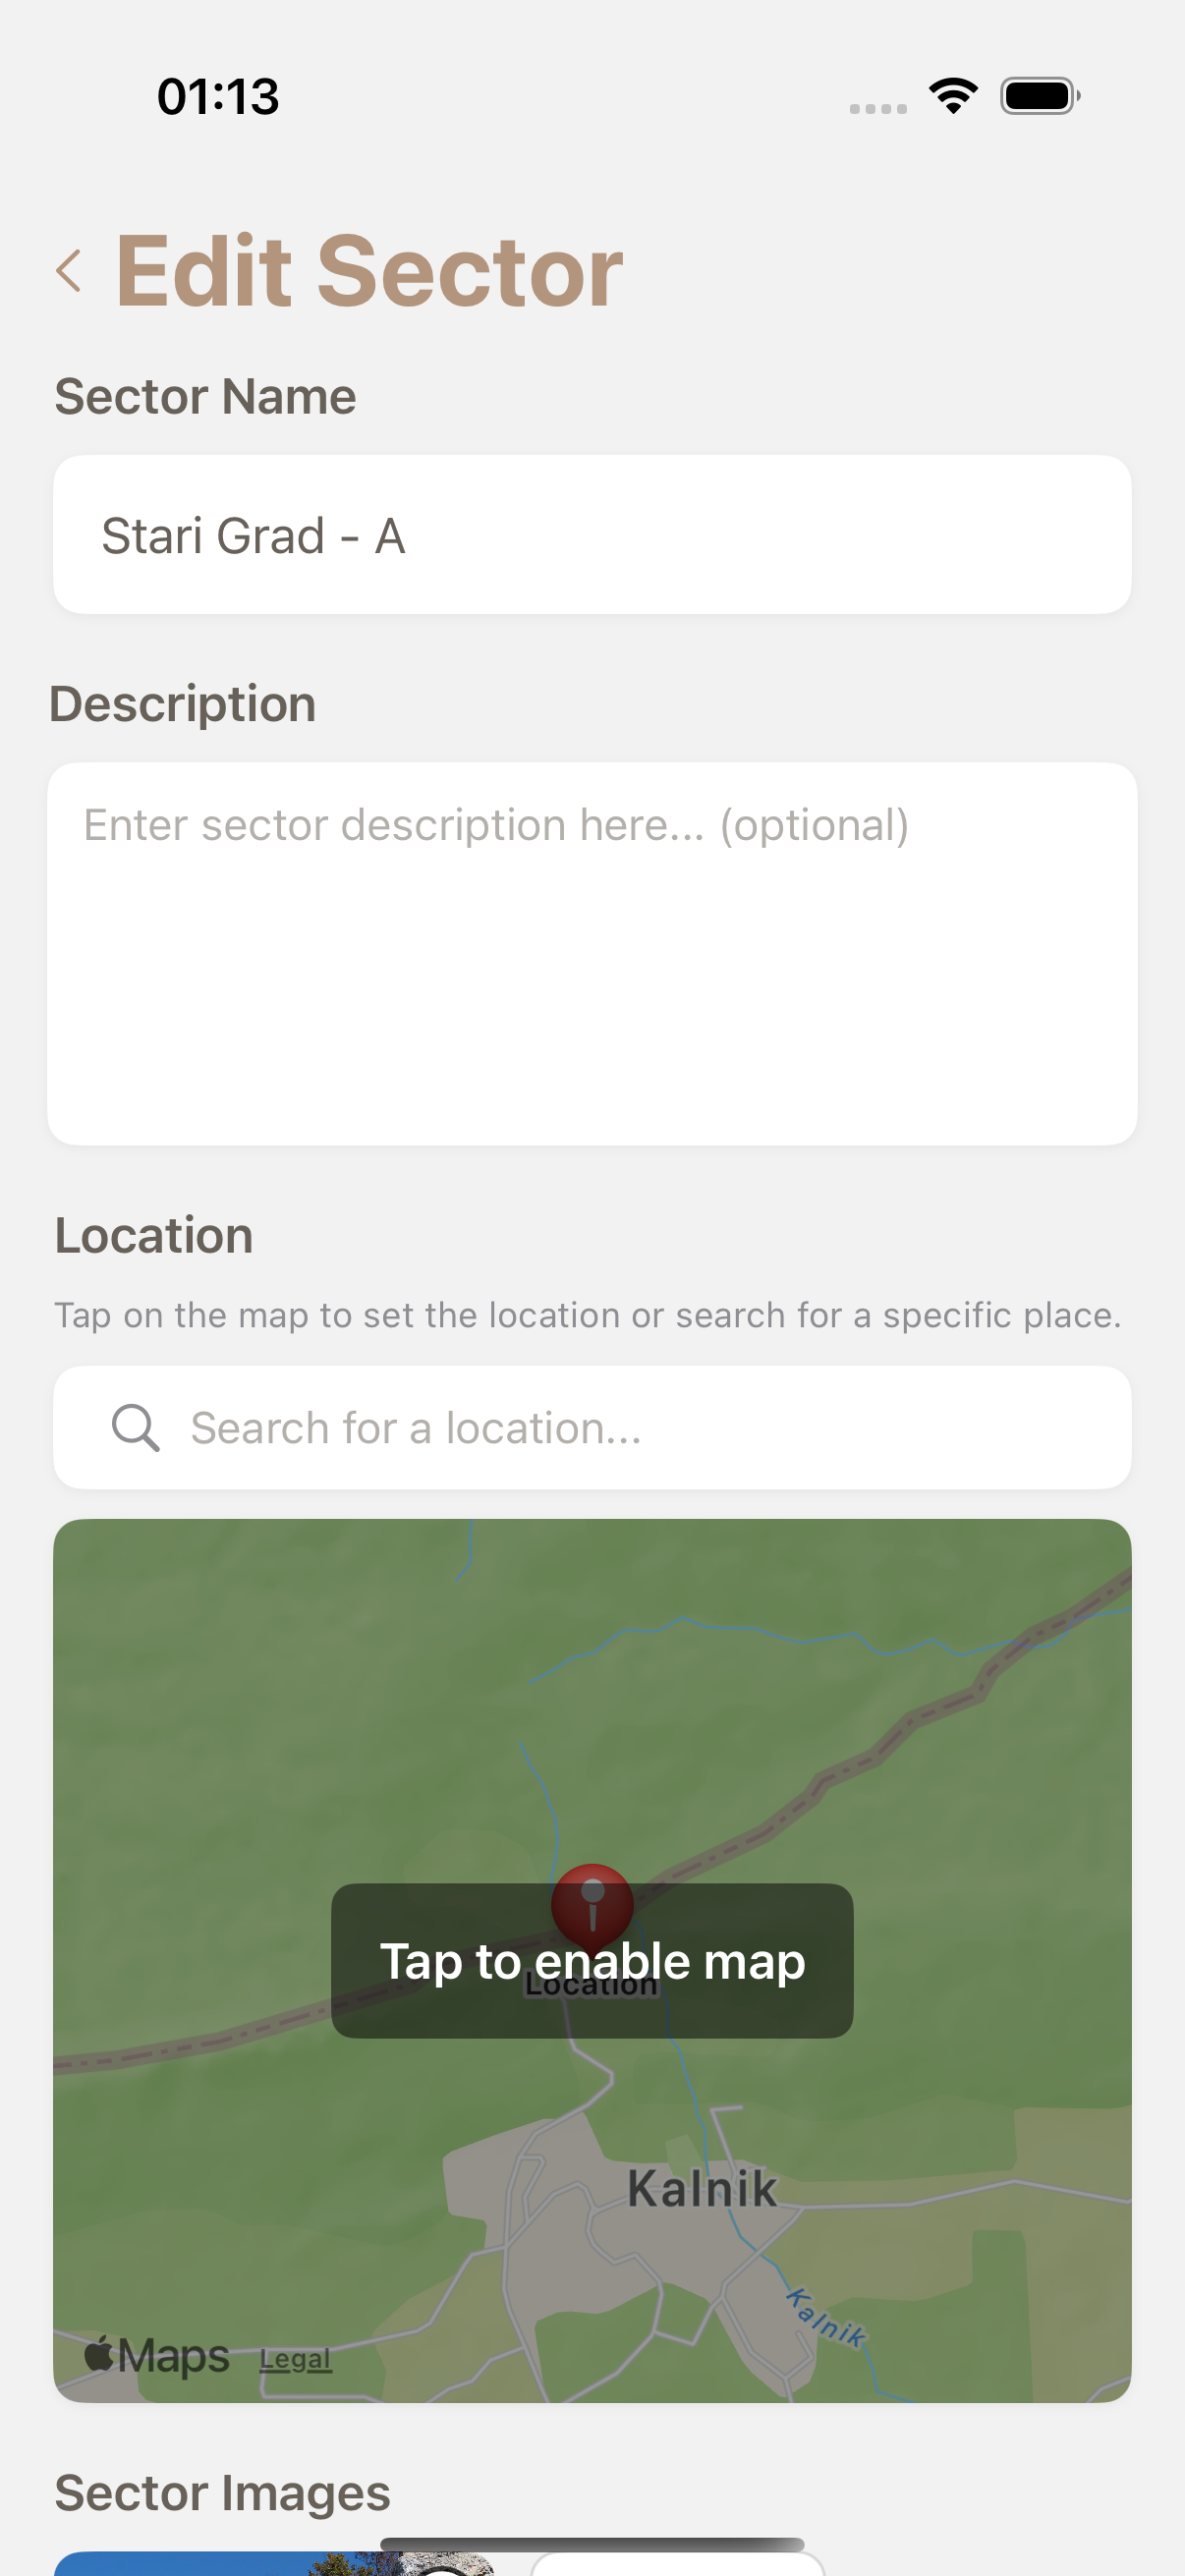
\includegraphics[width=\textwidth]{images/implementacija/editing-options/edit-sector.png}
        \caption{Mobilna aplikacija}
        \label{fig:uredjivanje_sektora_mob}
    \end{subfigure}
    \hfill
    \begin{subfigure}[b]{0.43\textwidth}
        \centering
        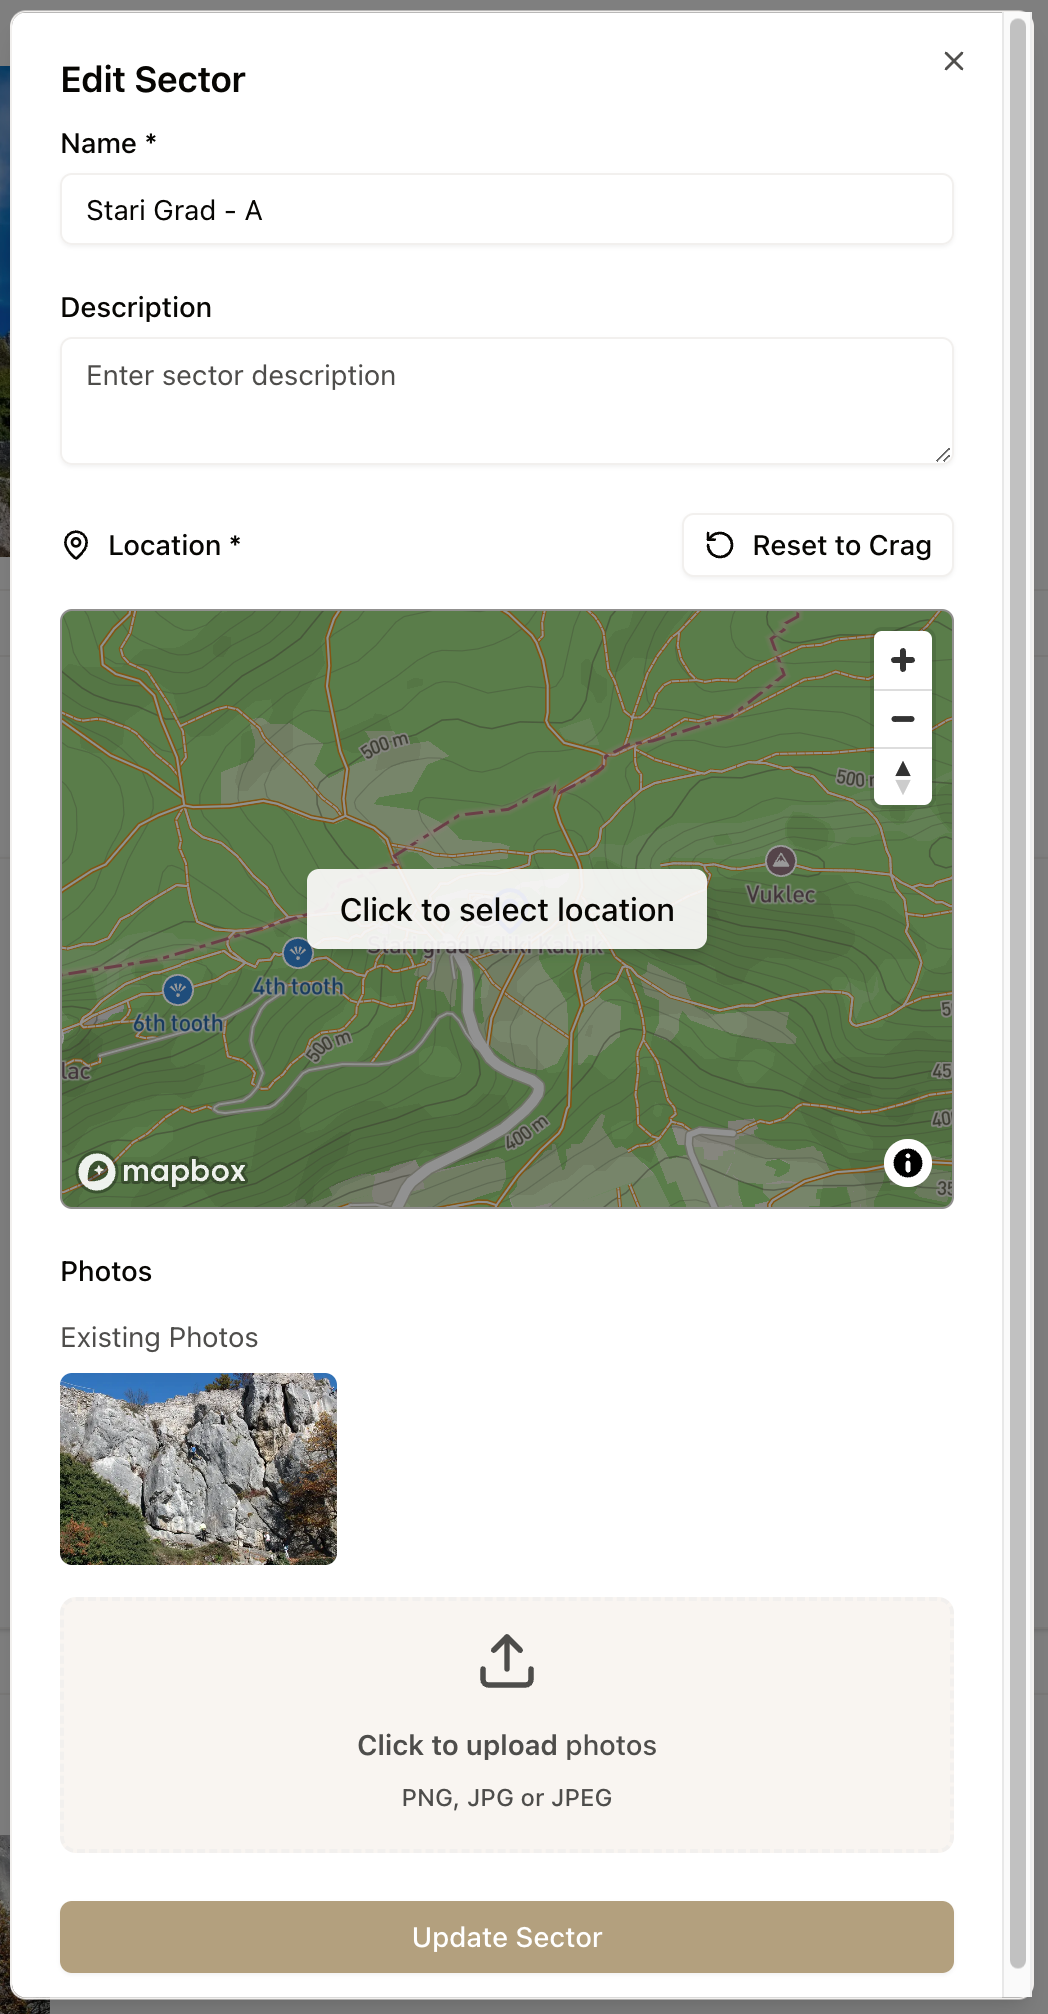
\includegraphics[width=\textwidth]{images/implementacija/web/editing-options/edit-sector.png}
        \caption{Web aplikacija}
        \label{fig:uredjivanje_sektora_web}
    \end{subfigure}
    \caption{Uređivanje postojećeg sektora}
    \label{fig:uredjivanje_sektora}
\end{figure}


\subsection{Dodavanje i uređivanje penjačkih smjerova}

Na najnižoj hijerarhijskoj razini nalazi se unos i uređivanje pojedinačnih penjačkih smjerova. Ovlašteni korisnici mogu dodavati nove penjačke smjerove unutar određenog sektora. Pristup ovoj funkcionalnosti omogućen je kroz izbornik na zaslonu s detaljnim pregledom penjačke lokacije sa označenim sektorom. Forma za kreiranje novog penjačkog smjera uključuje polja poput naziva, opisa, težine, tipa penjačkog smjera i dužine. Opcije za tip penjačkog smjera uključuju boulder, sportski, tradicionalni ili smjer s više penjačkih smjerova.

\begin{figure}[H]
    \centering
    \begin{subfigure}[b]{0.38\textwidth}
        \centering
        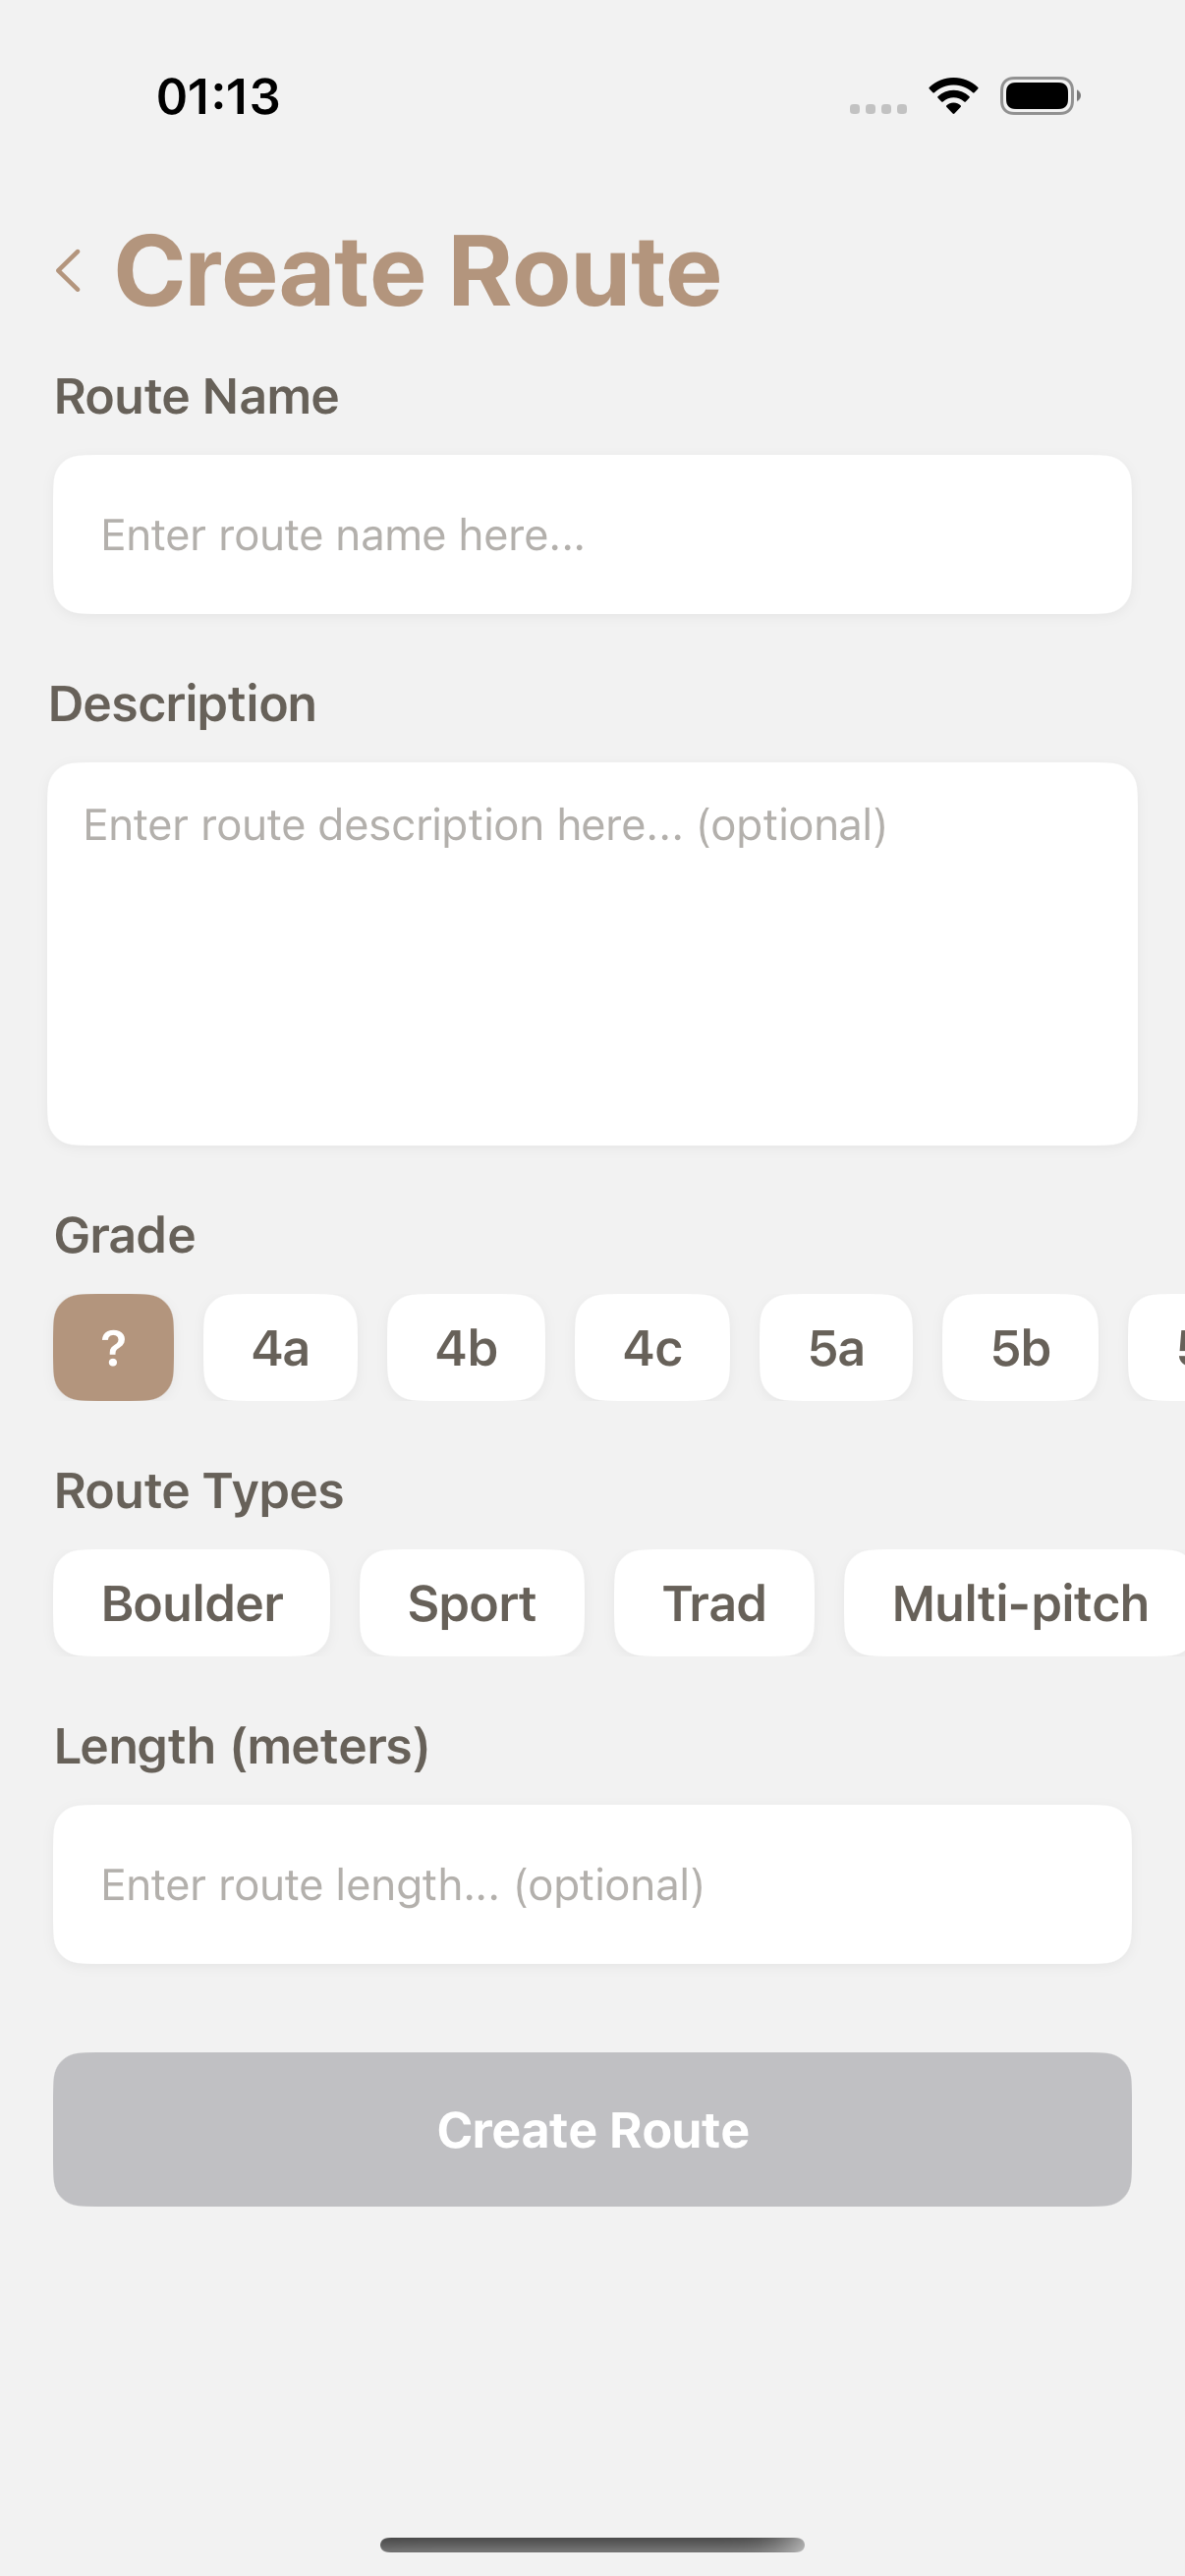
\includegraphics[width=\textwidth]{images/implementacija/editing-options/create-route.png}
        \caption{Mobilna aplikacija}
        \label{fig:dodavanje_smjera_mob}
    \end{subfigure}
    \hfill
    \begin{subfigure}[b]{0.43\textwidth}
        \centering
        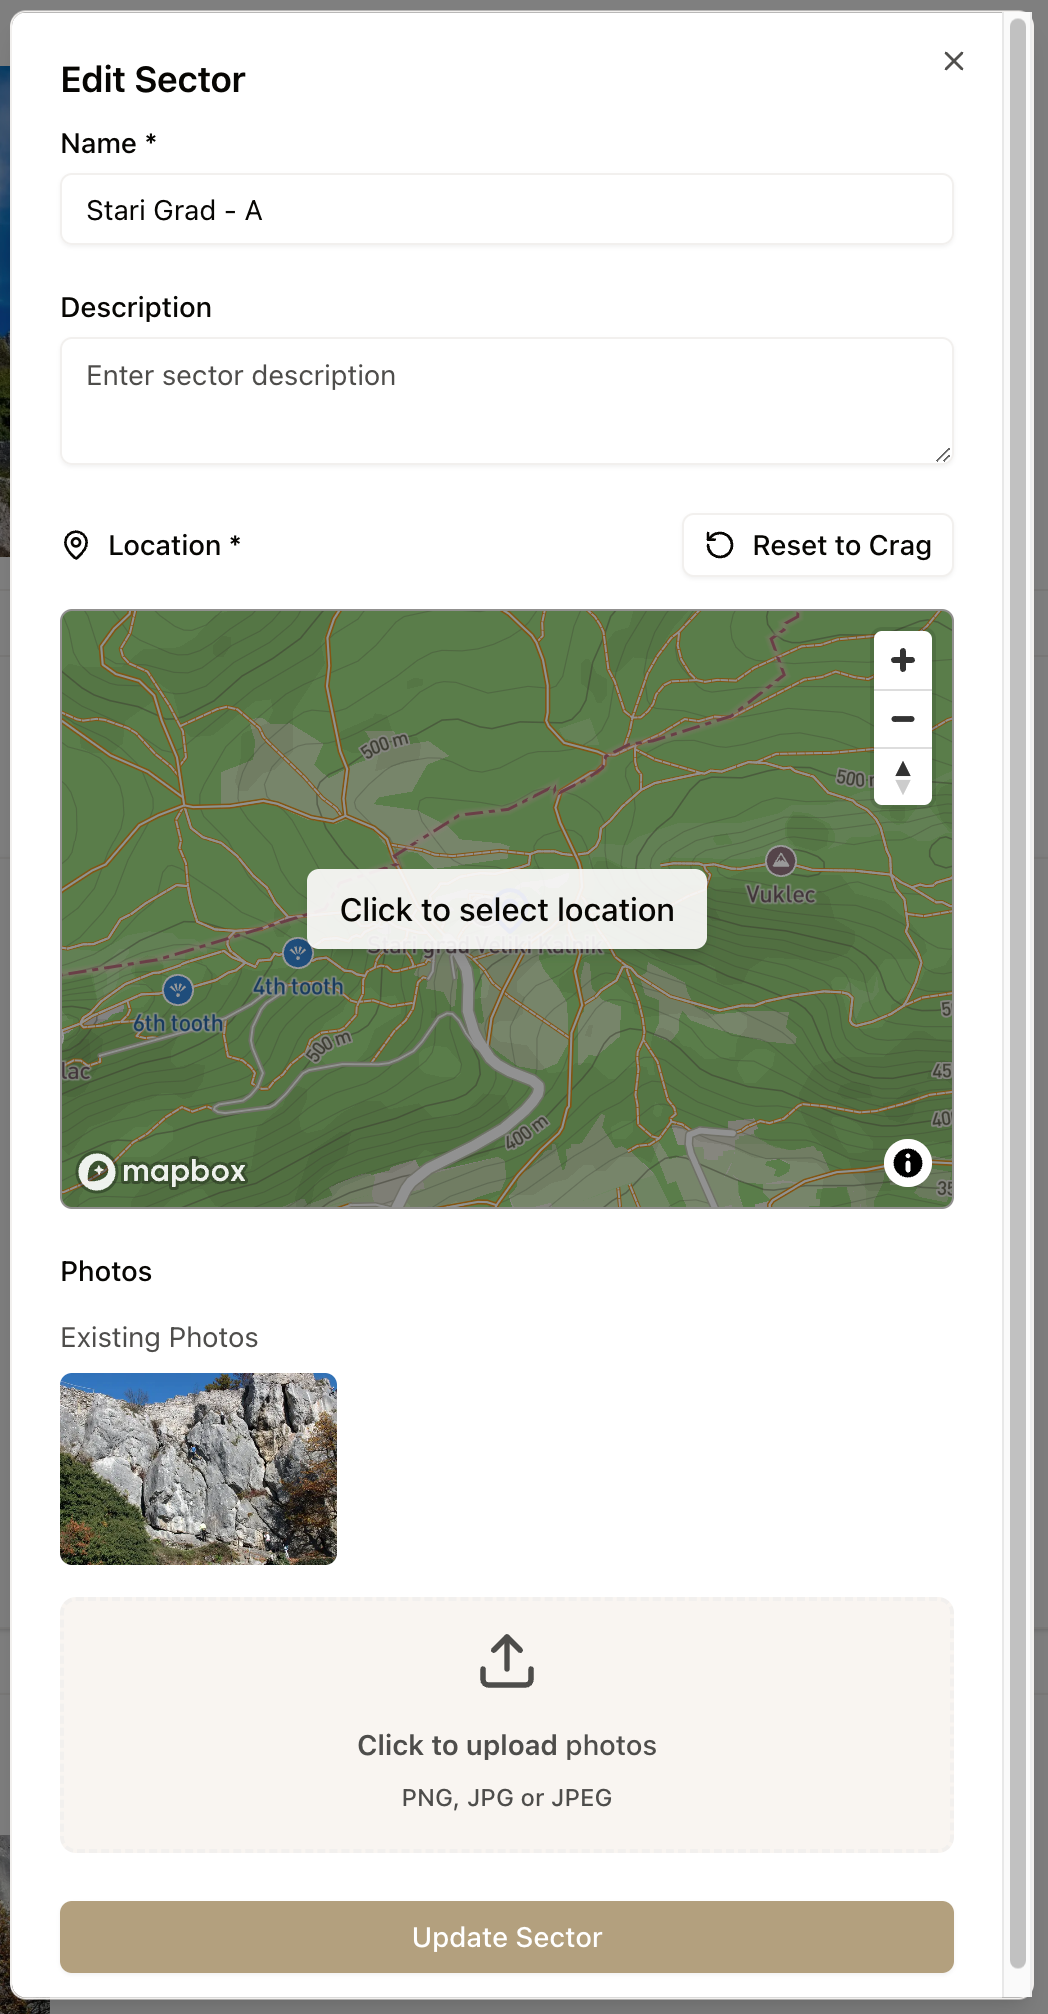
\includegraphics[width=\textwidth]{images/implementacija/web/editing-options/edit-sector.png}
        \caption{Web aplikacija}
        \label{fig:dodavanje_smjera_web}
    \end{subfigure}
    \caption{Dodavanje novog penjačkog smjera}
    \label{fig:dodavanje_smjera}
\end{figure}

Važno je primjetiti kako opcija dodavanja slike penjačkog smjera nije dostupna u formi za dodavanje novog penjačkog smjera i dostupan je samo na mobilnoj aplikaciji. Dodavanje fotografije je moguće nakon kreiranja penjačkog smjera u pregledu detalja penjačkog smjera. Klikom na izbornik u gornjem desnom kutu pregleda detalja penjačkog smjera, korisniku se prikazuje izbornik u kojem se nalazi opcija za dodavanje fotografije. Prvi korak u procesu dodavanja fotografije je slikanje fotografije penjačkog smjera pomoću kamere mobilnog uređaja. Nakon slikanja fotografije, korisniku se prikazuje slika na koju se može ručno ucrtati linija penjačkog smjera. Time je korisnik kreirao referentnu sliku penjačkog smjera koja se može koristiti za prepoznavanje penjačkog smjera.

TODO: DODATI SLIKE

\subsection{Uređivanje korisničkog profila}

Unutar korisničkog profila, u gornjem desnom kutu, nalazi se izbornik koji sadrži dodatne opcije za upravljanje računom i, ovisno o korisnikovim ovlastima, za doprinos sadržaju aplikacije. Odabirom opcije "Uredi profil" (eng. \textit{Edit profile}) korisnik odlazi na stranicu za uređivanje svojih podataka. Moguće je promijeniti ime, prezime, korisničko ime i datum rođenja. Aplikacija također omogućuje promjenu profilne fotografije te ažuriranje lozinke.

\begin{figure}[H]
    \centering
    \begin{subfigure}[b]{0.35\textwidth}
        \centering
        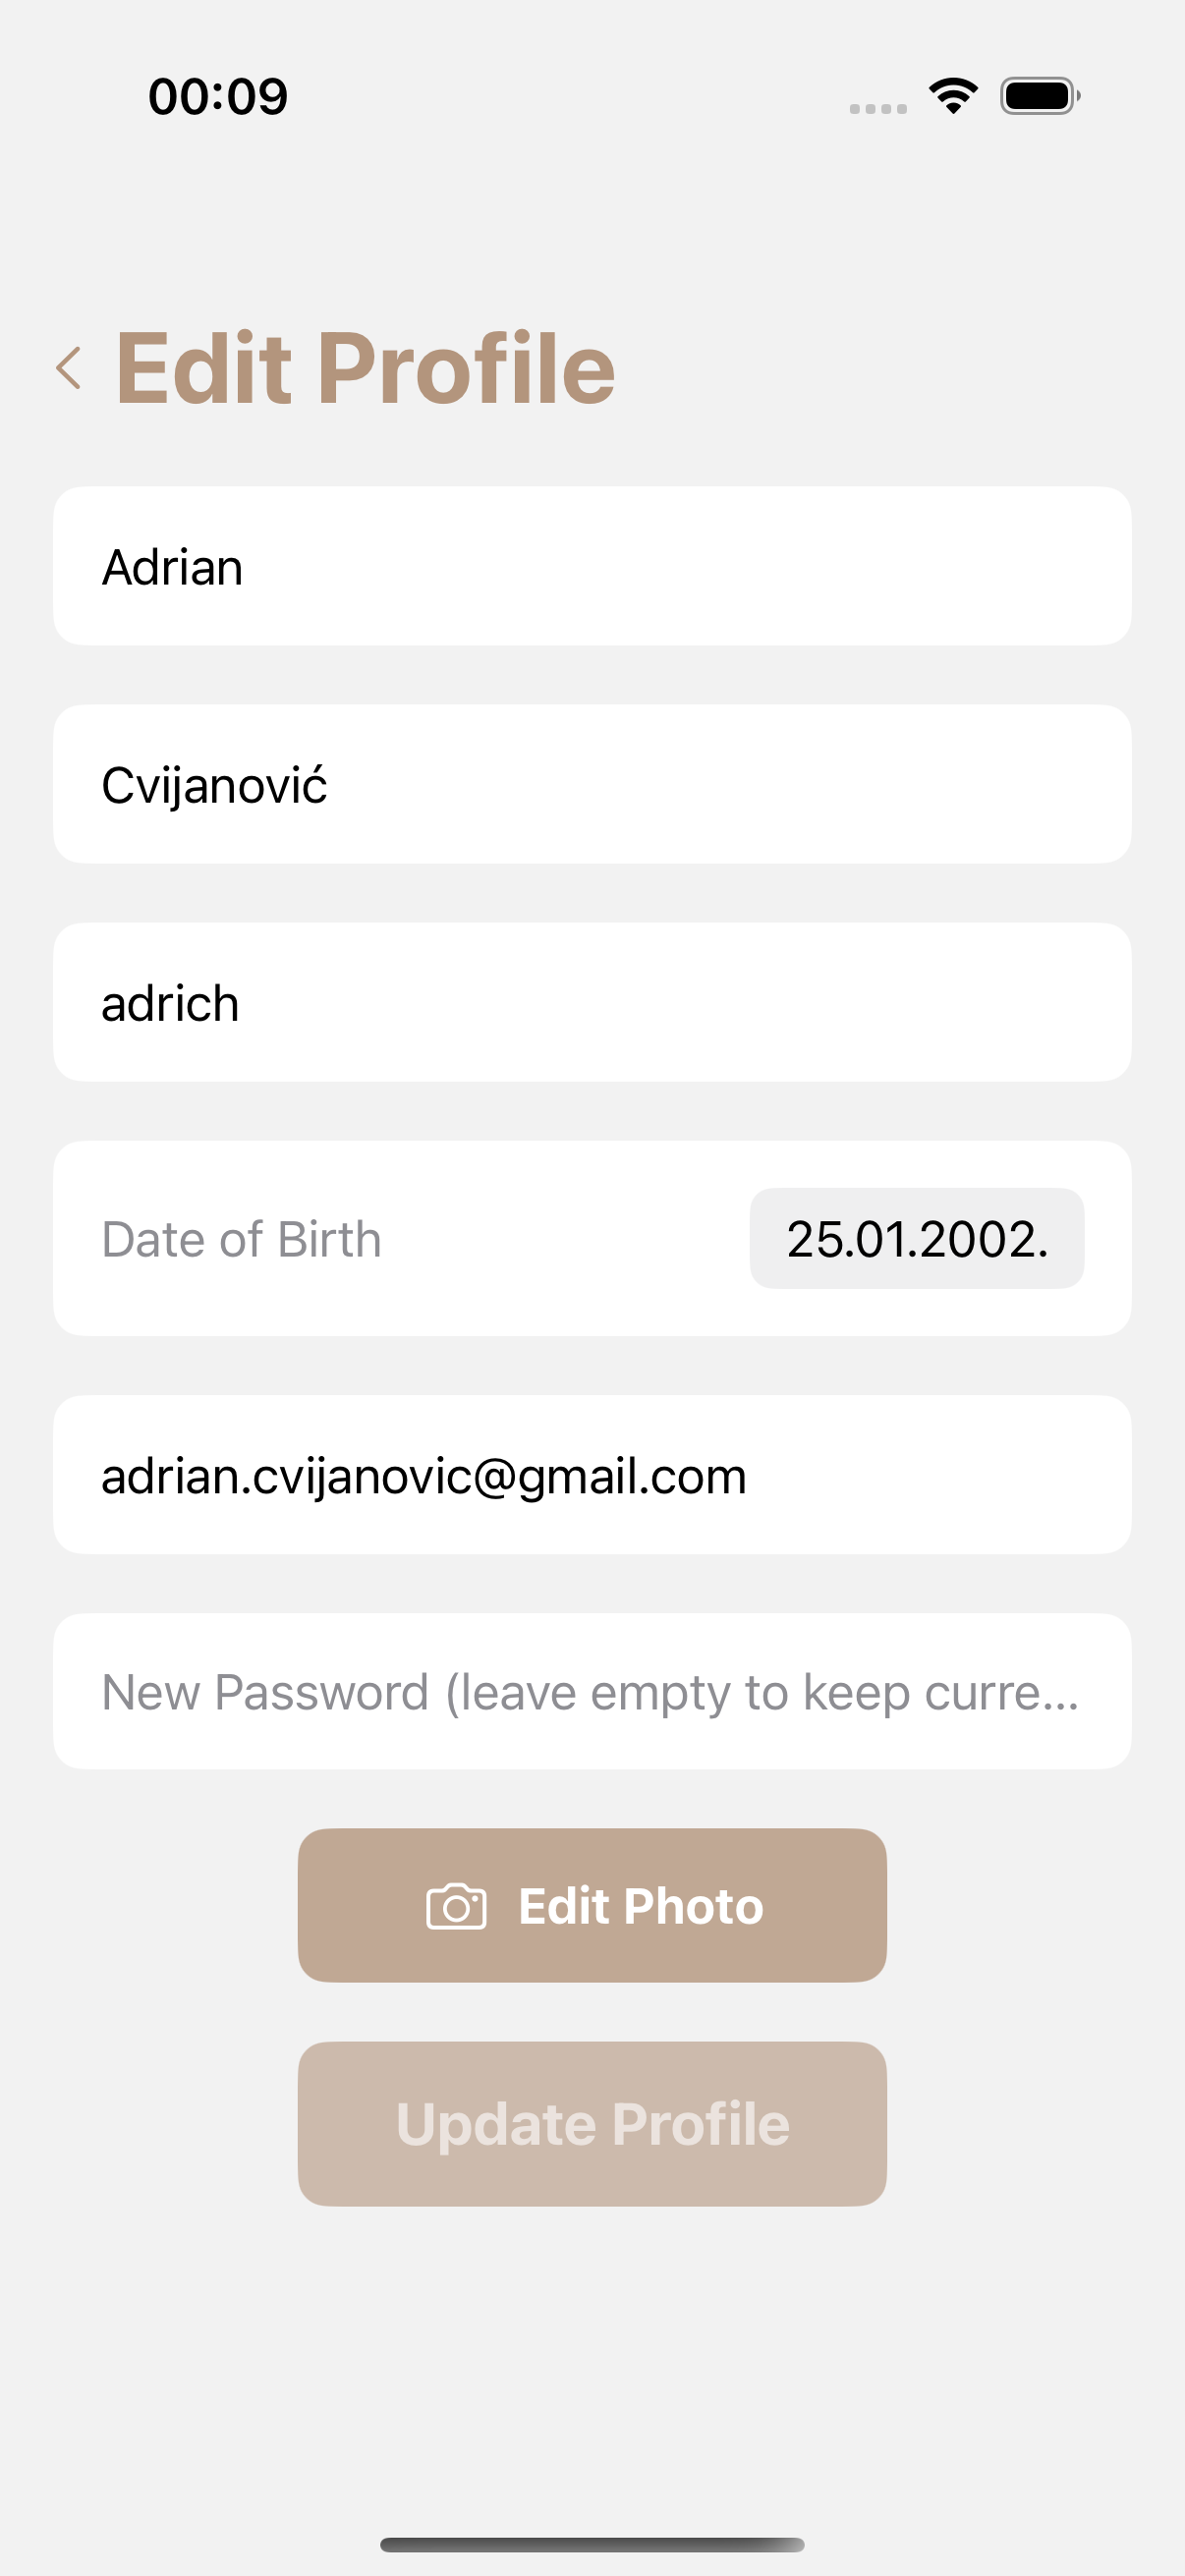
\includegraphics[width=\textwidth]{images/implementacija/editing-options/edit_profile.png}
        \caption{Mobilna aplikacija}
        \label{fig:uredjivanje_profila_mob}
    \end{subfigure}
    \hfill
    \begin{subfigure}[b]{0.55\textwidth}
        \centering
        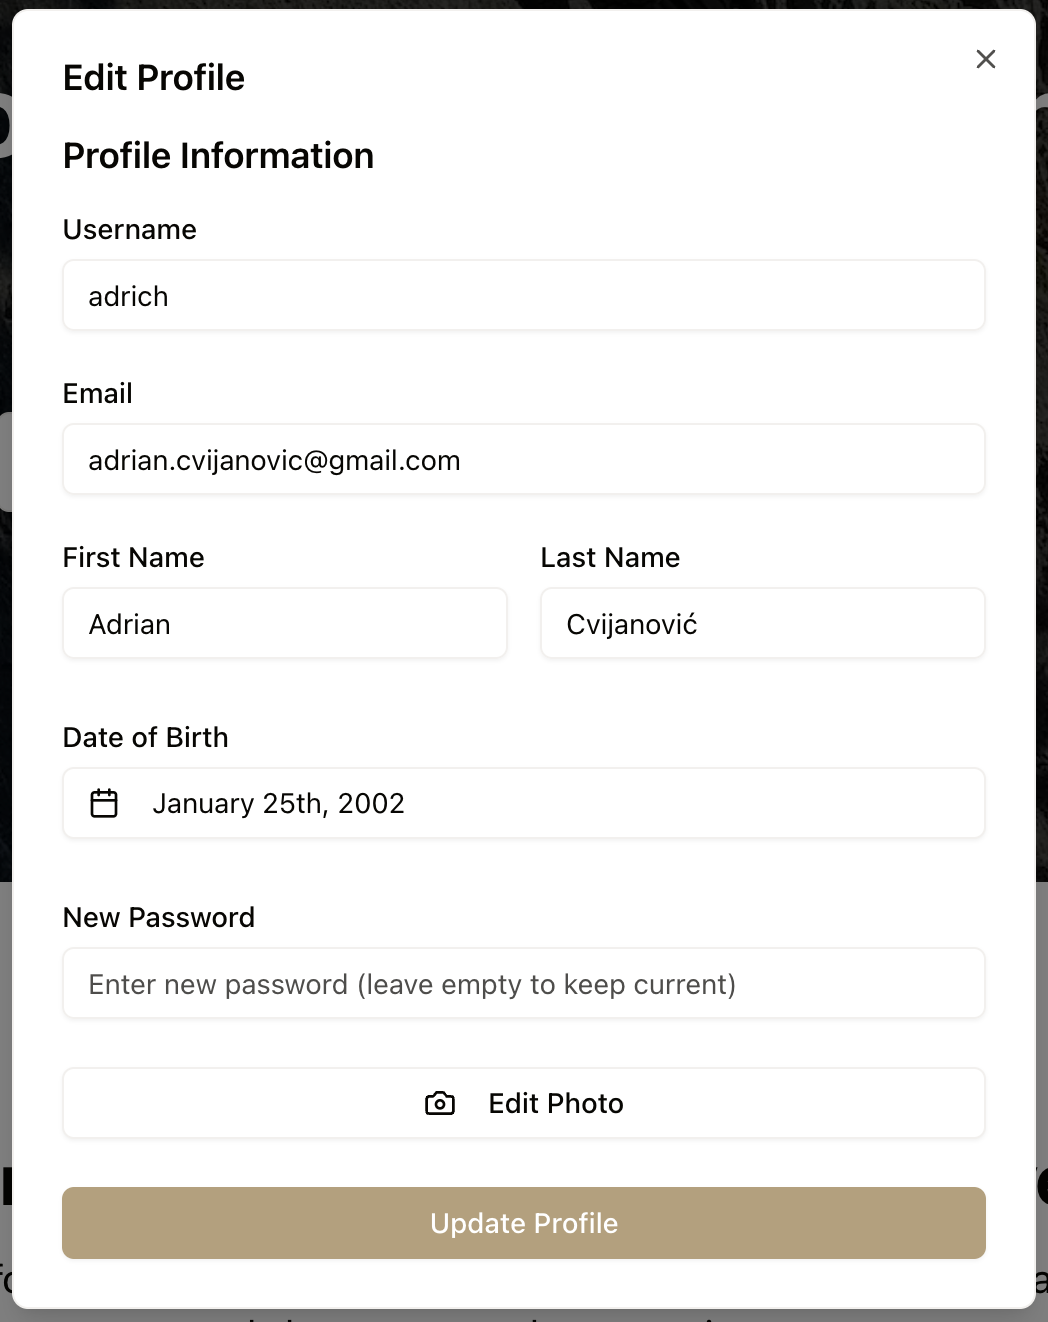
\includegraphics[width=\textwidth]{images/implementacija/web/editing-options/edit-user.png}
        \caption{Web aplikacija}
        \label{fig:uredjivanje_profila_web}
    \end{subfigure}
    \caption{Uređivanje korisničkog profila}
    \label{fig:uredjivanje_profila}
\end{figure}